\documentclass[10pt]{beamer}
\usepackage[utf8]{inputenc}
\usepackage[russian]{babel}
\usepackage{amsmath}
\usepackage{amsfonts}
\usepackage{amssymb}
\usepackage{caption}
\usepackage{subcaption}
\usepackage{graphicx}
\usepackage{textcomp}
\usepackage{placeins}
\usetheme{Dresden}
\expandafter\def\expandafter\insertshorttitle\expandafter{%
	\insertshorttitle\hfill%
	\insertframenumber\,/\,\inserttotalframenumber}

\makeatletter
\newenvironment{withoutheadline}{
	\setbeamertemplate{headline}[default]
	\def\beamer@entrycode{\vspace*{-\headheight}}
}{}

\begin{document}
\title{Управление движением группы мобильных роботов}
\author{Хафизов Х.А.}
\begin{withoutheadline}
\begin{frame}
	
	\begin{figure}
		\centering
		
\includegraphics[width=0.2\linewidth]{others/SPbSPU_Logo}
		\label{fig:spbspulogo}
	\end{figure}
	\begin{center}

	\small Санкт-Петербургский политехнический университет Петра Великого \\
	Кафедра "Механика и процессы управления" \\
	mc.spbstu.ru\par
	\bigskip
	\usebeamerfont{title}\usebeamercolor{title}Управление движением группы мобильных роботов \\
	\end{center}
	\begin{columns}[T]%beamer
		\column{0.45\textwidth}
		\column{0.55\textwidth}
		\begin{description}
			\item[Выполнил:] Хафизов Х.А.
			\item[Начный рук.:] проф. Бурдаков С.Ф.
		\end{description}
	\end{columns}
	
\end{frame}
\end{withoutheadline}
\begin{frame}
	\frametitle{Содержание}
	\tableofcontents
\end{frame}
\section{Введение}
\begin{frame}
	\frametitle{Управление квадрокоптером}
	Объект управления — квадрокоптер. БПЛА с высоким потенциалом. \par
	\bigskip
	Сферы применения:\par
	\begin{itemize}
		\item Наблюдение и контроль зон, поражённых естественными и техногенными катастрофами
		\item Спасательные операции
		\item Метеорология
		\item Военные цели
	\end{itemize}
	\bigskip
	Подходы к решению задачи управления одиночным квадрокоптером хорошо изучены. 
	
\end{frame}
\begin{frame}
	\frametitle{Управление группой квадрокоптеров}
	Преимущества группы квадрокоптеров перед одиночным роботом:
	\begin{itemize}
		\item Увеличение надёжности системы
		\item Расширение спектра задач
	\end{itemize}
	\bigskip
	Существующие подходы:
	\begin{itemize}
		\item Централизованная стратегия
		\item Децентрализованная стратегия
	\end{itemize}
 	\begin{columns}
	\column{0.5\textwidth}
	\begin{figure}
		\centering
		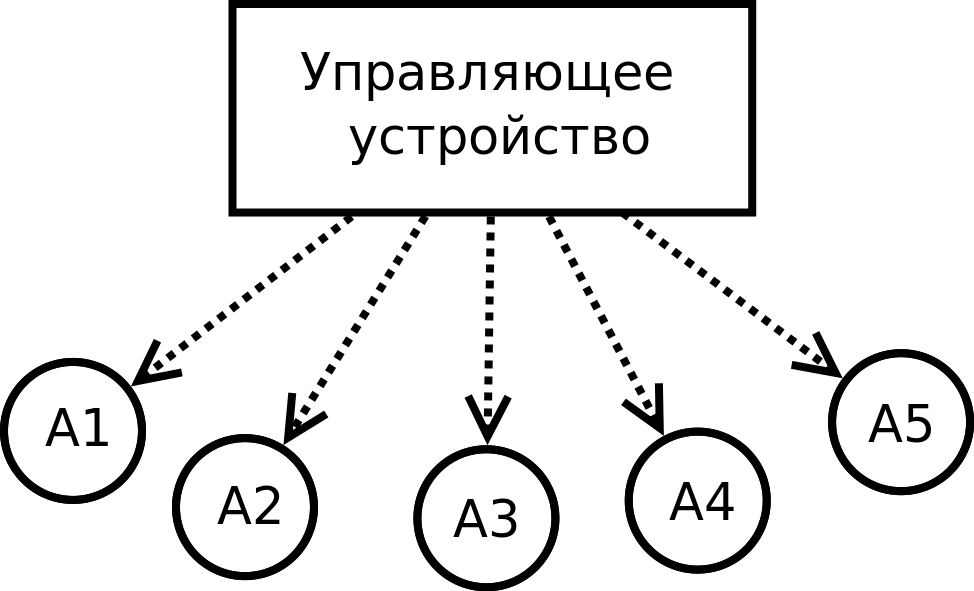
\includegraphics[width=0.8\linewidth]{others/centr-platoon-controll2}
		\caption{Централизованная стратегия}
		\label{fig:centr-platoon-controll}
	\end{figure}
	\column{0.5\textwidth}
	\begin{figure}
		\centering
		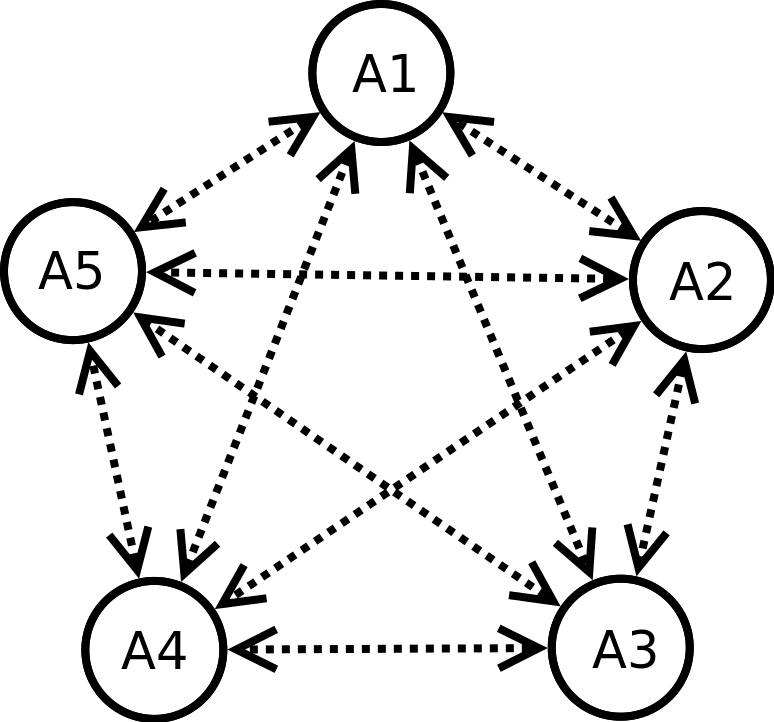
\includegraphics[width=0.63\linewidth]{others/decen-platoon-collective}
		\caption{Децентрализованная стратегия}
		\label{fig:decen-platoon-collective}
	\end{figure}
\end{columns}
\end{frame}
\begin{frame}
	\frametitle{Строевая задача}
	Управление строем — частный случай группового управления. Отличие — фиксированное положение агентов в пространстве.
	Каждый участник строя здесь и далее называется агентом.
\begin{figure}
	
	\centering
	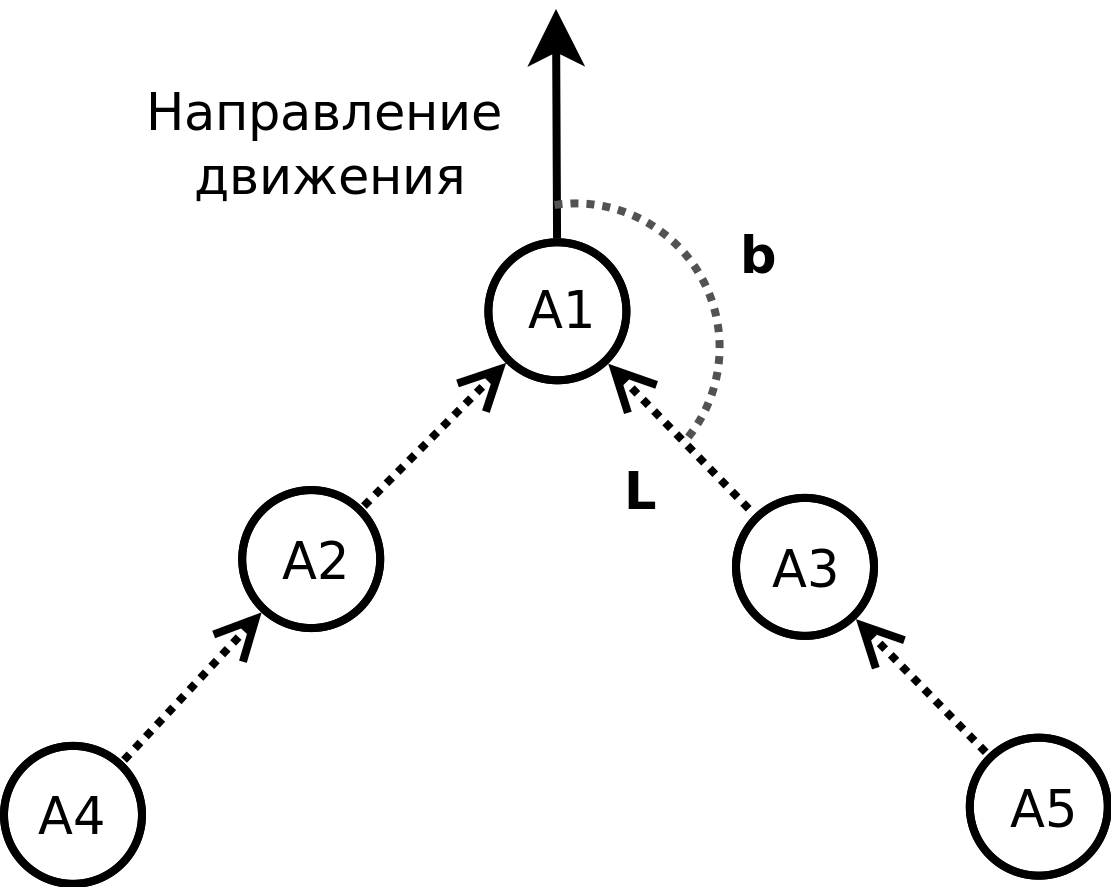
\includegraphics[width=0.40\linewidth]{platoon/wedge-platoon-prez}
	\caption{Строй в форме клина из 5-ти агентов}
	\label{fig:wedge-platoon-prez}
\end{figure}
Задачи: видеомониторинг, разведка, формирование ФАР, картирование сельскохозяйственных угодий.
\end{frame}
\section{Постановка задачи}
\begin{frame}
	\frametitle{Постановка задачи}
	Разработать алгоритм децентрализованного управления строем квадракоптеров. Моделирование будет происходить в горизонтальной плоскости $xy$ \par
	\bigskip
	Каждый квадракоптер:
	\begin{itemize}
		\item Имеет массу $m=1\text{кг}$
		\item Имеет ограниченную тягу двигателя $F_{max}$
		\item Имеет ограниченную зону радиовидимости $R_a$
	\end{itemize}
	\bigskip
	Задача которая ставится перед строем — движение по траектории с задаваемой скоростью.
\end{frame}
\begin{frame}
	\frametitle{Требования к решению}
	\begin{itemize}
		\item Алгоритм устойчив к малым возмущениям и к отклонениям по начальным условиям
		\item При потере целостности строя из-за сильного возмущения выполнение задачи должно быть продолжено
		\item Отказ любого агента не оказывает критического влияния на выполнение задачи
	\end{itemize}
\end{frame}
\section{Алгоритм}
\begin{frame}
	\frametitle{Общее описание алгоритма}
	Агенты в строю разделяются на два типа:
	\begin{itemize}
		\item Мастер — движется по траектории
		\item Миньон — формирует своё местоположение относительно других агентов так, чтобы поддерживать рисунок строя
	\end{itemize}
\end{frame}
\begin{frame}
	\frametitle{Алгоритм управления мастера}
	Закон управления мастера состоит из двух компонент:
	$$ \vec{u} = \vec{u}_{along} + \vec{u}_{across} $$
	$$  |\vec{u}_{along}| \sim |\vec{\upsilon}_{d} - \vec{\upsilon}| \text{, направлена вдоль траектории} $$
	$$  \vec{u}_{across} \text{ — пропорциональна перпендикуляру к траектории} $$
	
	\begin{columns}
	\column{0.5\textwidth}
	\begin{figure}
		\centering
		
\includegraphics[width=0.8\linewidth]{master-trajectory-0}
		\caption{След движения агента по траектории}
		\label{fig:master-trajectory-0}
	\end{figure}
	\column{0.5\textwidth}
	\begin{figure}
		\centering
		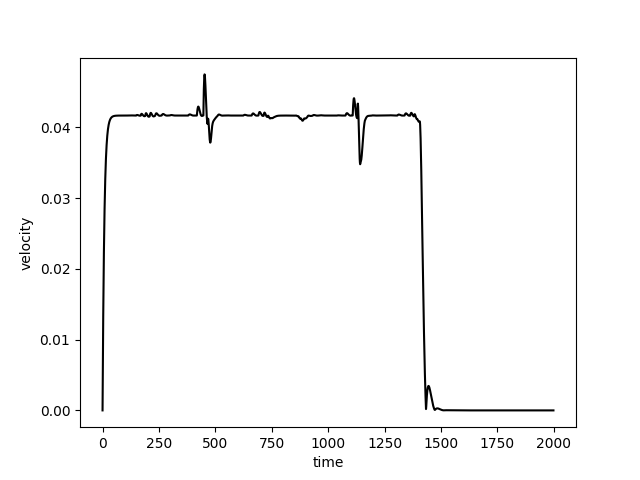
\includegraphics[width=0.8\linewidth]{master-trajectory-0-velocity}
		\caption{Скорость агента при движении. $\vec{\upsilon}_{d} = 20 \text{м/c}$}
		\label{fig:master-trajectory-0-velocity}
	\end{figure}
\end{columns}
\end{frame}
\begin{frame}
	\frametitle{Алгоритм управления миньона}
	Задача — формировать своё местоположение относительно других агентов так, чтобы сохранялся рисунок строя.
	\begin{columns}
		\column{0.5\textwidth}
		
		\begin{figure}
			\centering
			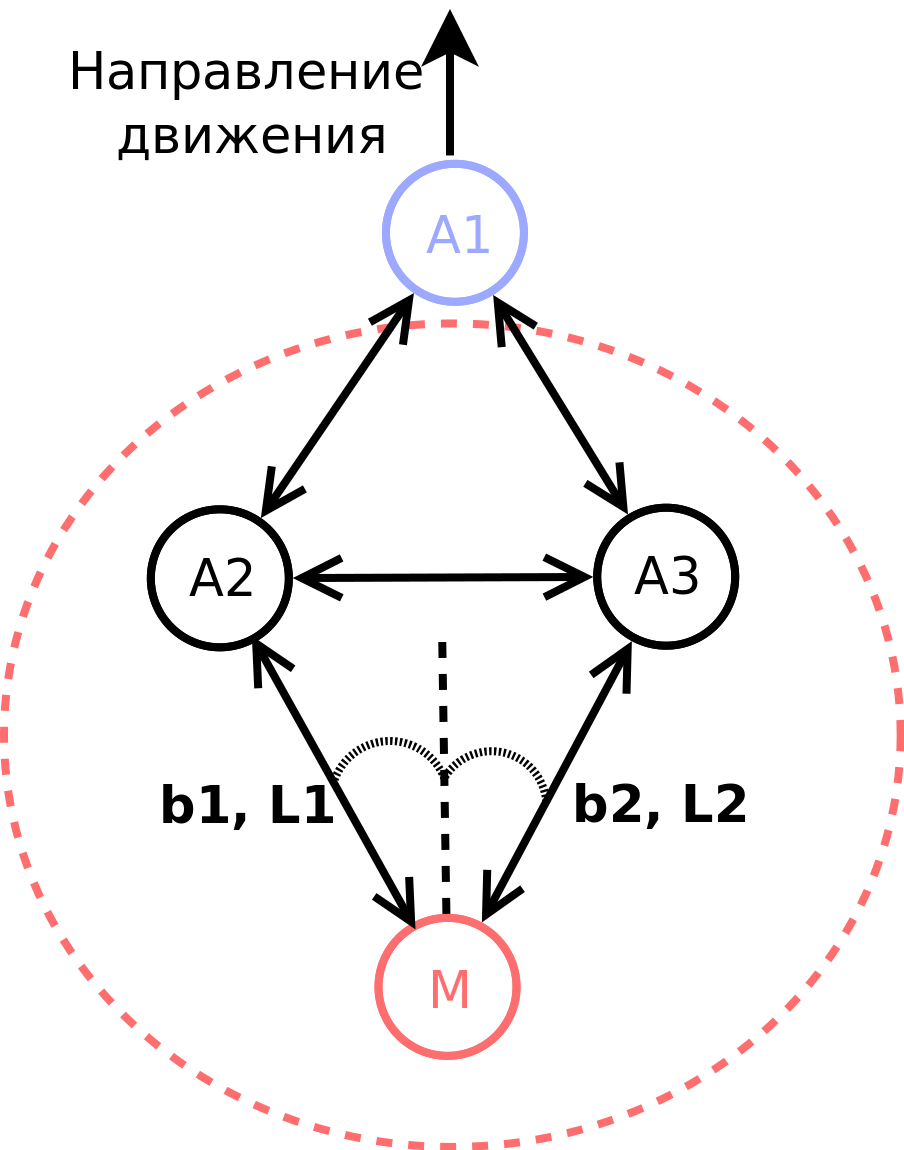
\includegraphics[width=0.8\linewidth]{others/minions-alg}
			\caption{Миньон в строю}
			\label{fig:minions-alg}
		\end{figure}
		\column{0.5\textwidth}
		
		\begin{figure}
			\centering
			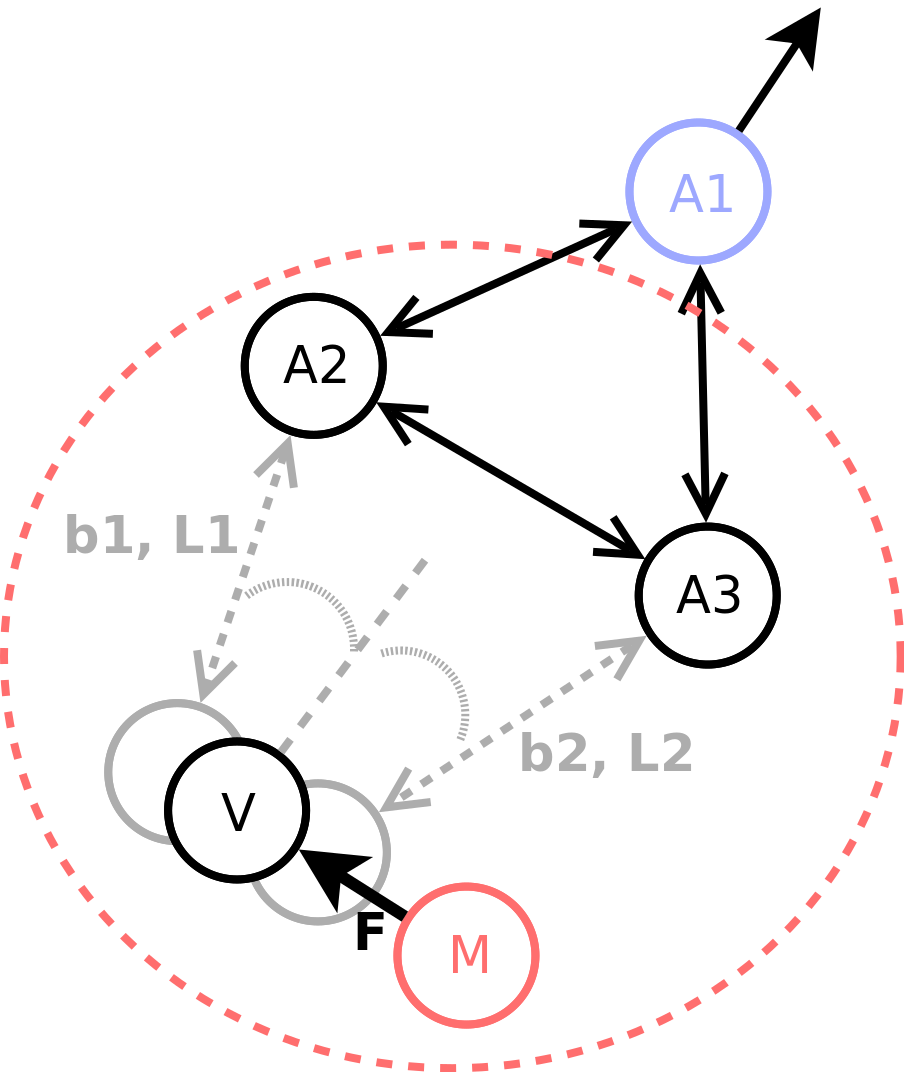
\includegraphics[width=0.8\linewidth]{others/minions-alg-rotated}
			\caption{Миньон в повернувшемся строю}
			\label{fig:minions-alg-rotated}
		\end{figure}
	\end{columns}
\end{frame}
\section{Результаты}
\begin{frame}
	\frametitle{Движение строя без возмущений}
	Движение строя из 9-ти агентов в форме окружности по спиралевидной траектории. Мастером является агент в центре окружности.
	\begin{columns}
		\column{0.5\textwidth}
		\begin{figure}
			\centering
			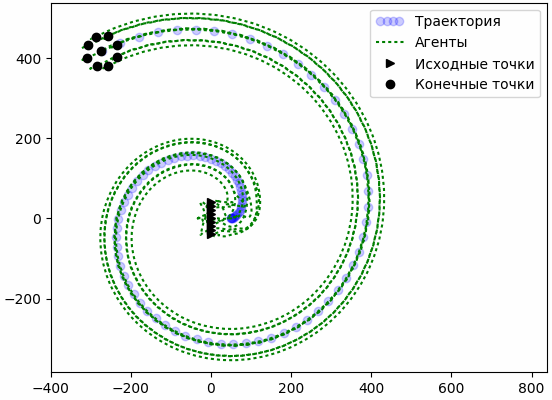
\includegraphics[width=1\linewidth]{others/circle-platoon}
			\caption{Общий план}
			\label{fig:circle-platoon}
		\end{figure}
		\column{0.5\textwidth}
		\begin{figure}
			\centering
			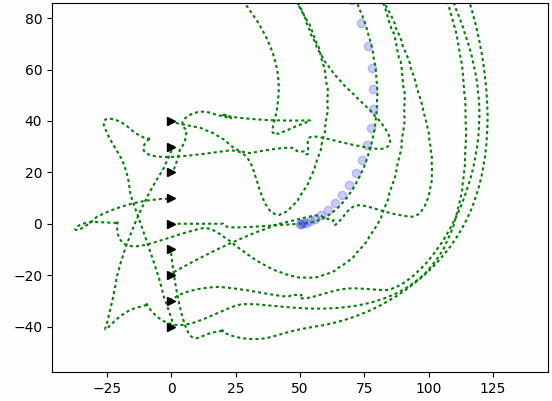
\includegraphics[width=1\linewidth]{others/circle-platoon-zoom1}
			\caption{Процесс формирования строя}
			\label{fig:circle-platoon-zoom1}
		\end{figure}
	\end{columns}
\end{frame}
\begin{frame}
	\frametitle{Движение строя при малых возмущениях}
	\begin{figure}
		\centering
		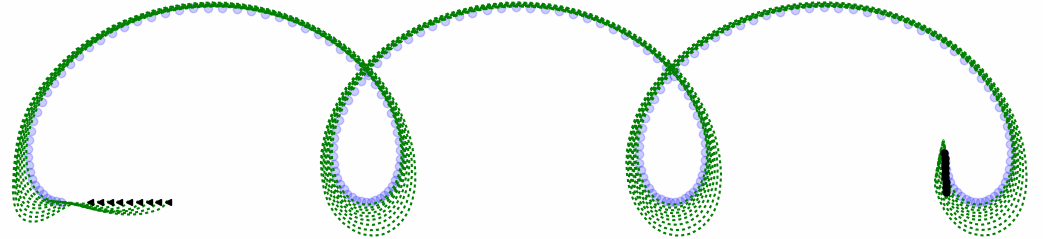
\includegraphics[width=0.9\linewidth]{platoon/line-platoon-cropped}
		\caption{Движение строя в виде линии из 9-ти агентов}
		\label{fig:line-platoon-cropped}
	\end{figure}
	\begin{figure}
		\centering
		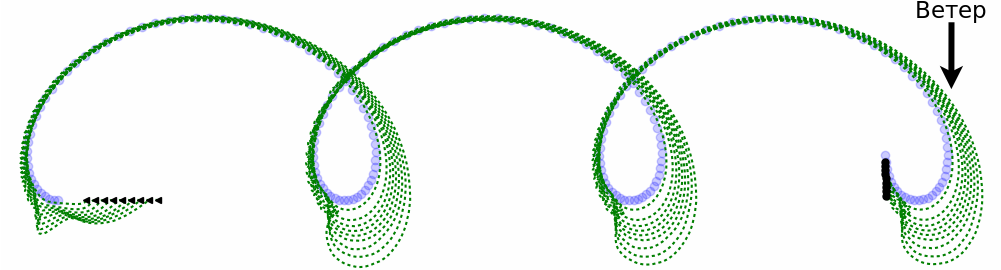
\includegraphics[width=0.9\linewidth]{platoon/line-platoon-winded-cropped-txt}
		\caption{Движение строя при постоянном южном ветре}
		\label{fig:line-platoon-winded-cropped-txt}
	\end{figure}
\end{frame}
\begin{frame}
	\frametitle{Движение строя при отказах агентов}
	Движение строя из 5-ти агентов в форме линии перпендикулярной к траектории с отказом мастера и миньона.
	\begin{columns}
		\column{0.5\textwidth}
		\begin{figure}
			\centering
			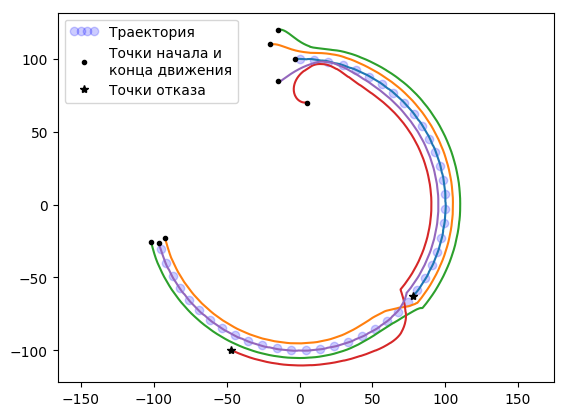
\includegraphics[width=1\linewidth]{platoon/with-crashes}
			\caption{Общий план}
			\label{fig:with-crashes}
		\end{figure}
		\column{0.5\textwidth}
		\begin{figure}
			\centering
			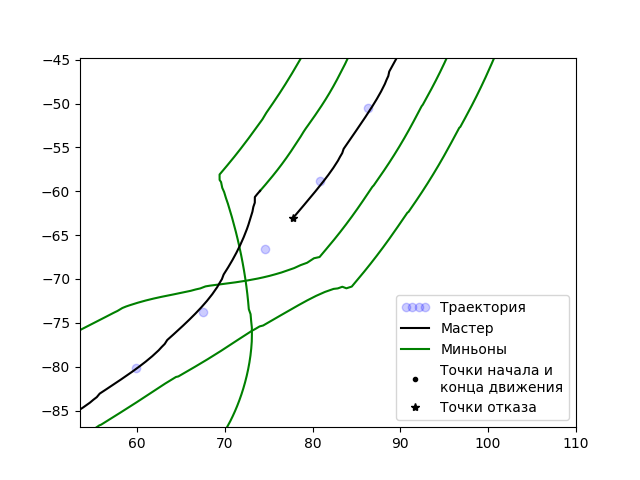
\includegraphics[width=1\linewidth]{platoon/with-crashes-zoom3}
			\caption{Отказ мастера}
			\label{fig:with-crashes-zoom3}
		\end{figure}
	\end{columns}
\end{frame}
\begin{frame}
	\frametitle{Движение строя при отказах агентов (подробнее)}
	\begin{columns}
	\column{0.5\textwidth}
		\begin{figure}
			\centering
			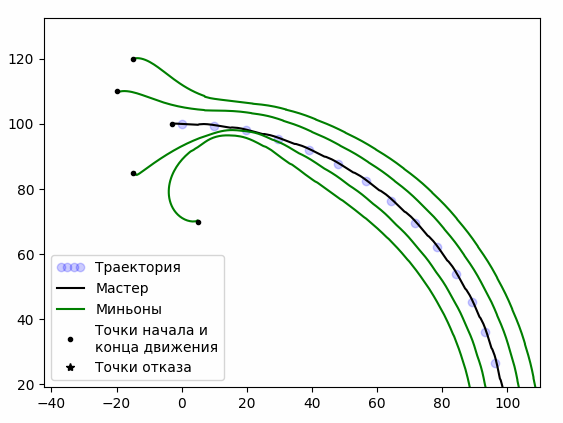
\includegraphics[width=1\linewidth]{platoon/with-crashes-zoom2}
			\caption{Формирование строя}
			\label{fig:with-crashes-zoom2}
		\end{figure}
	\column{0.5\textwidth}
		\begin{figure}
			\centering
			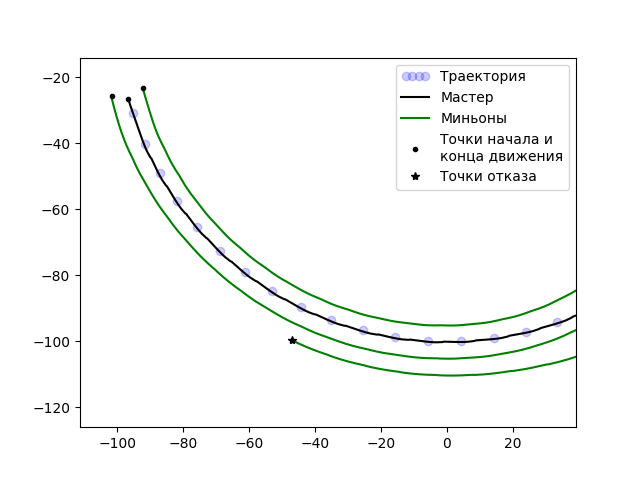
\includegraphics[width=1\linewidth]{platoon/with-crashes-zoom1}
			\caption{Отказ миньона}
			\label{fig:with-crashes-zoom1}
		\end{figure}
	\end{columns}
\end{frame}

\begin{frame}
	\frametitle{Движение строя при критических возмущениях}
	Строй из-за сильного возмущения, подействовавшего на двух агентов теряет свою целостность.
	\begin{columns}
		\column{0.5\textwidth}
		\begin{figure}
			\centering
			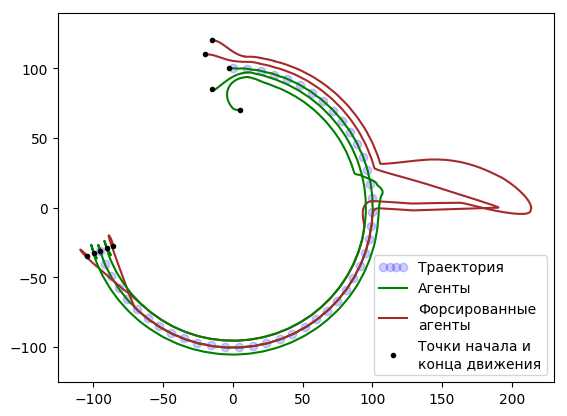
\includegraphics[width=1\linewidth]{platoon/with-bird}
			\caption{Общий план}
			\label{fig:with-bird}
		\end{figure}
		\column{0.5\textwidth}
		Образуются две подгруппы — 2 и 3 агента.\par Области радиовидимости не пересекаются.
		\begin{figure}
			\centering
			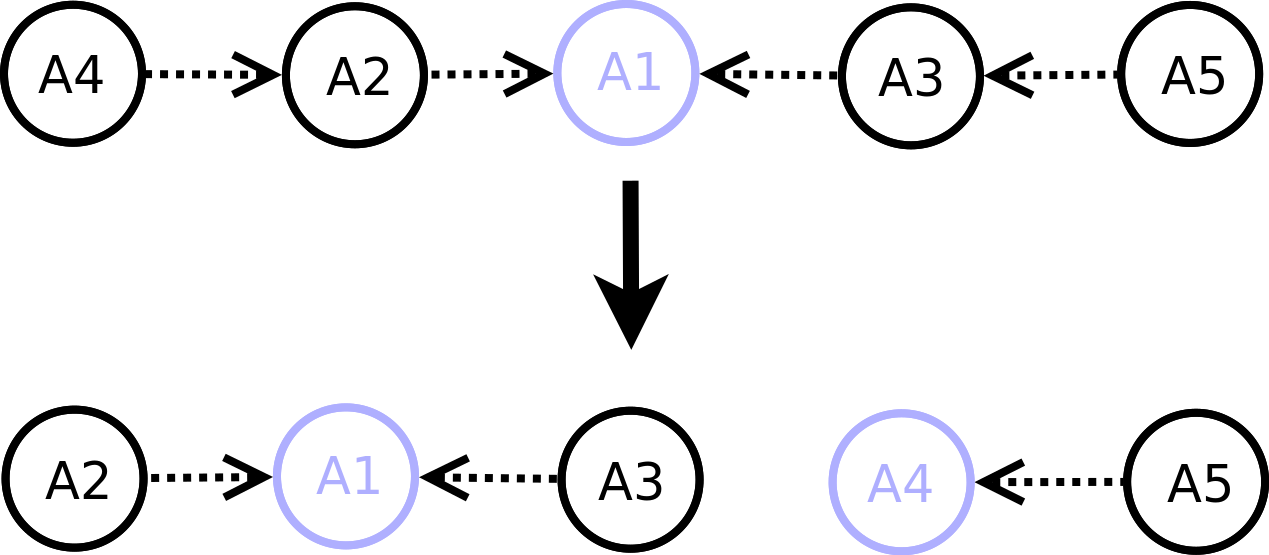
\includegraphics[width=1\linewidth]{platoon/with-bird-to-groups}
			\caption{Разбиение строя на подгруппы}
			\label{fig:with-bird-to-groups}
		\end{figure} 	
	\end{columns}
\end{frame}
\begin{frame}
	\frametitle{Движение строя при критических возмущениях (подробнее)}
	\begin{columns}
		\column{0.5\textwidth}
			\begin{figure}
				\centering
				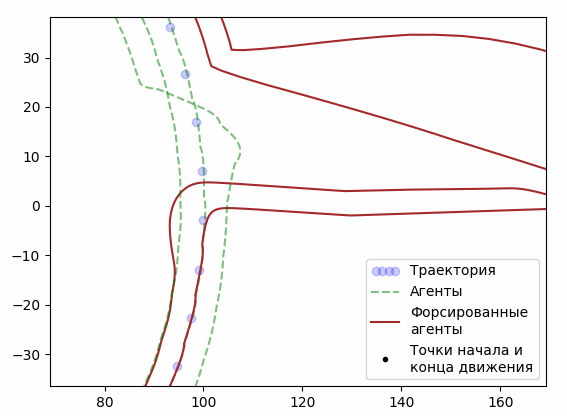
\includegraphics[width=1\linewidth]{platoon/with-bird-zoom1}
				\caption{Возврат на траекторию}
				\label{fig:with-bird-zoom1}
			\end{figure}
		\column{0.5\textwidth}
			\begin{figure}
				\centering
				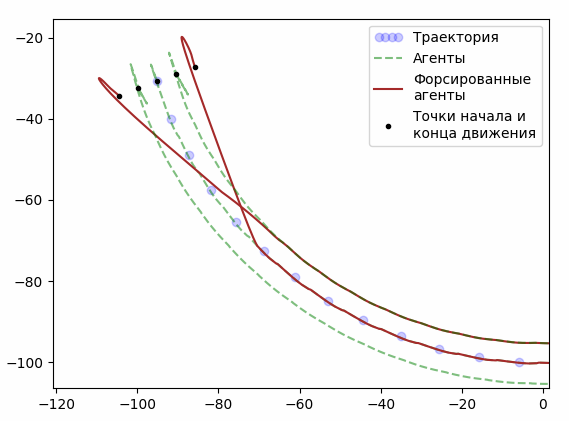
\includegraphics[width=1\linewidth]{platoon/with-bird-zoom2}
				\caption{Восстановление строя}
				\label{fig:with-bird-zoom2}
			\end{figure}
	\end{columns}
\end{frame}
\section{Заключение}
\begin{frame}
	\frametitle{Выводы}
	Реализованный децентрализованный алгоритм управления строем обладает следующими характеристиками:
	\begin{itemize}
		\item Малые возмущения приводят к малым отклонениям строя от желаемого закона движения
		\item Алгоритм управления устойчив к отклонениям по начальным условиям
		\item Потеря целостности и отказ агентов не приводит к невыполнению задачи
		\item Высокая масштабируемость относительно количества агентов в строю  
	\end{itemize}
\end{frame}
\begin{frame}
	
  \begin{minipage}[t][.8\textheight]{\textwidth}
  	\vspace{3cm}
	\begin{center}
		\large Спасибо за внимание!
	\end{center}
	
	\vfill
	
    \footnotesize https://github.com/xozzslip/agents-platooning
\end{minipage}
\end{frame}

\begin{frame}[noframenumbering]
\begin{figure}
	\centering
	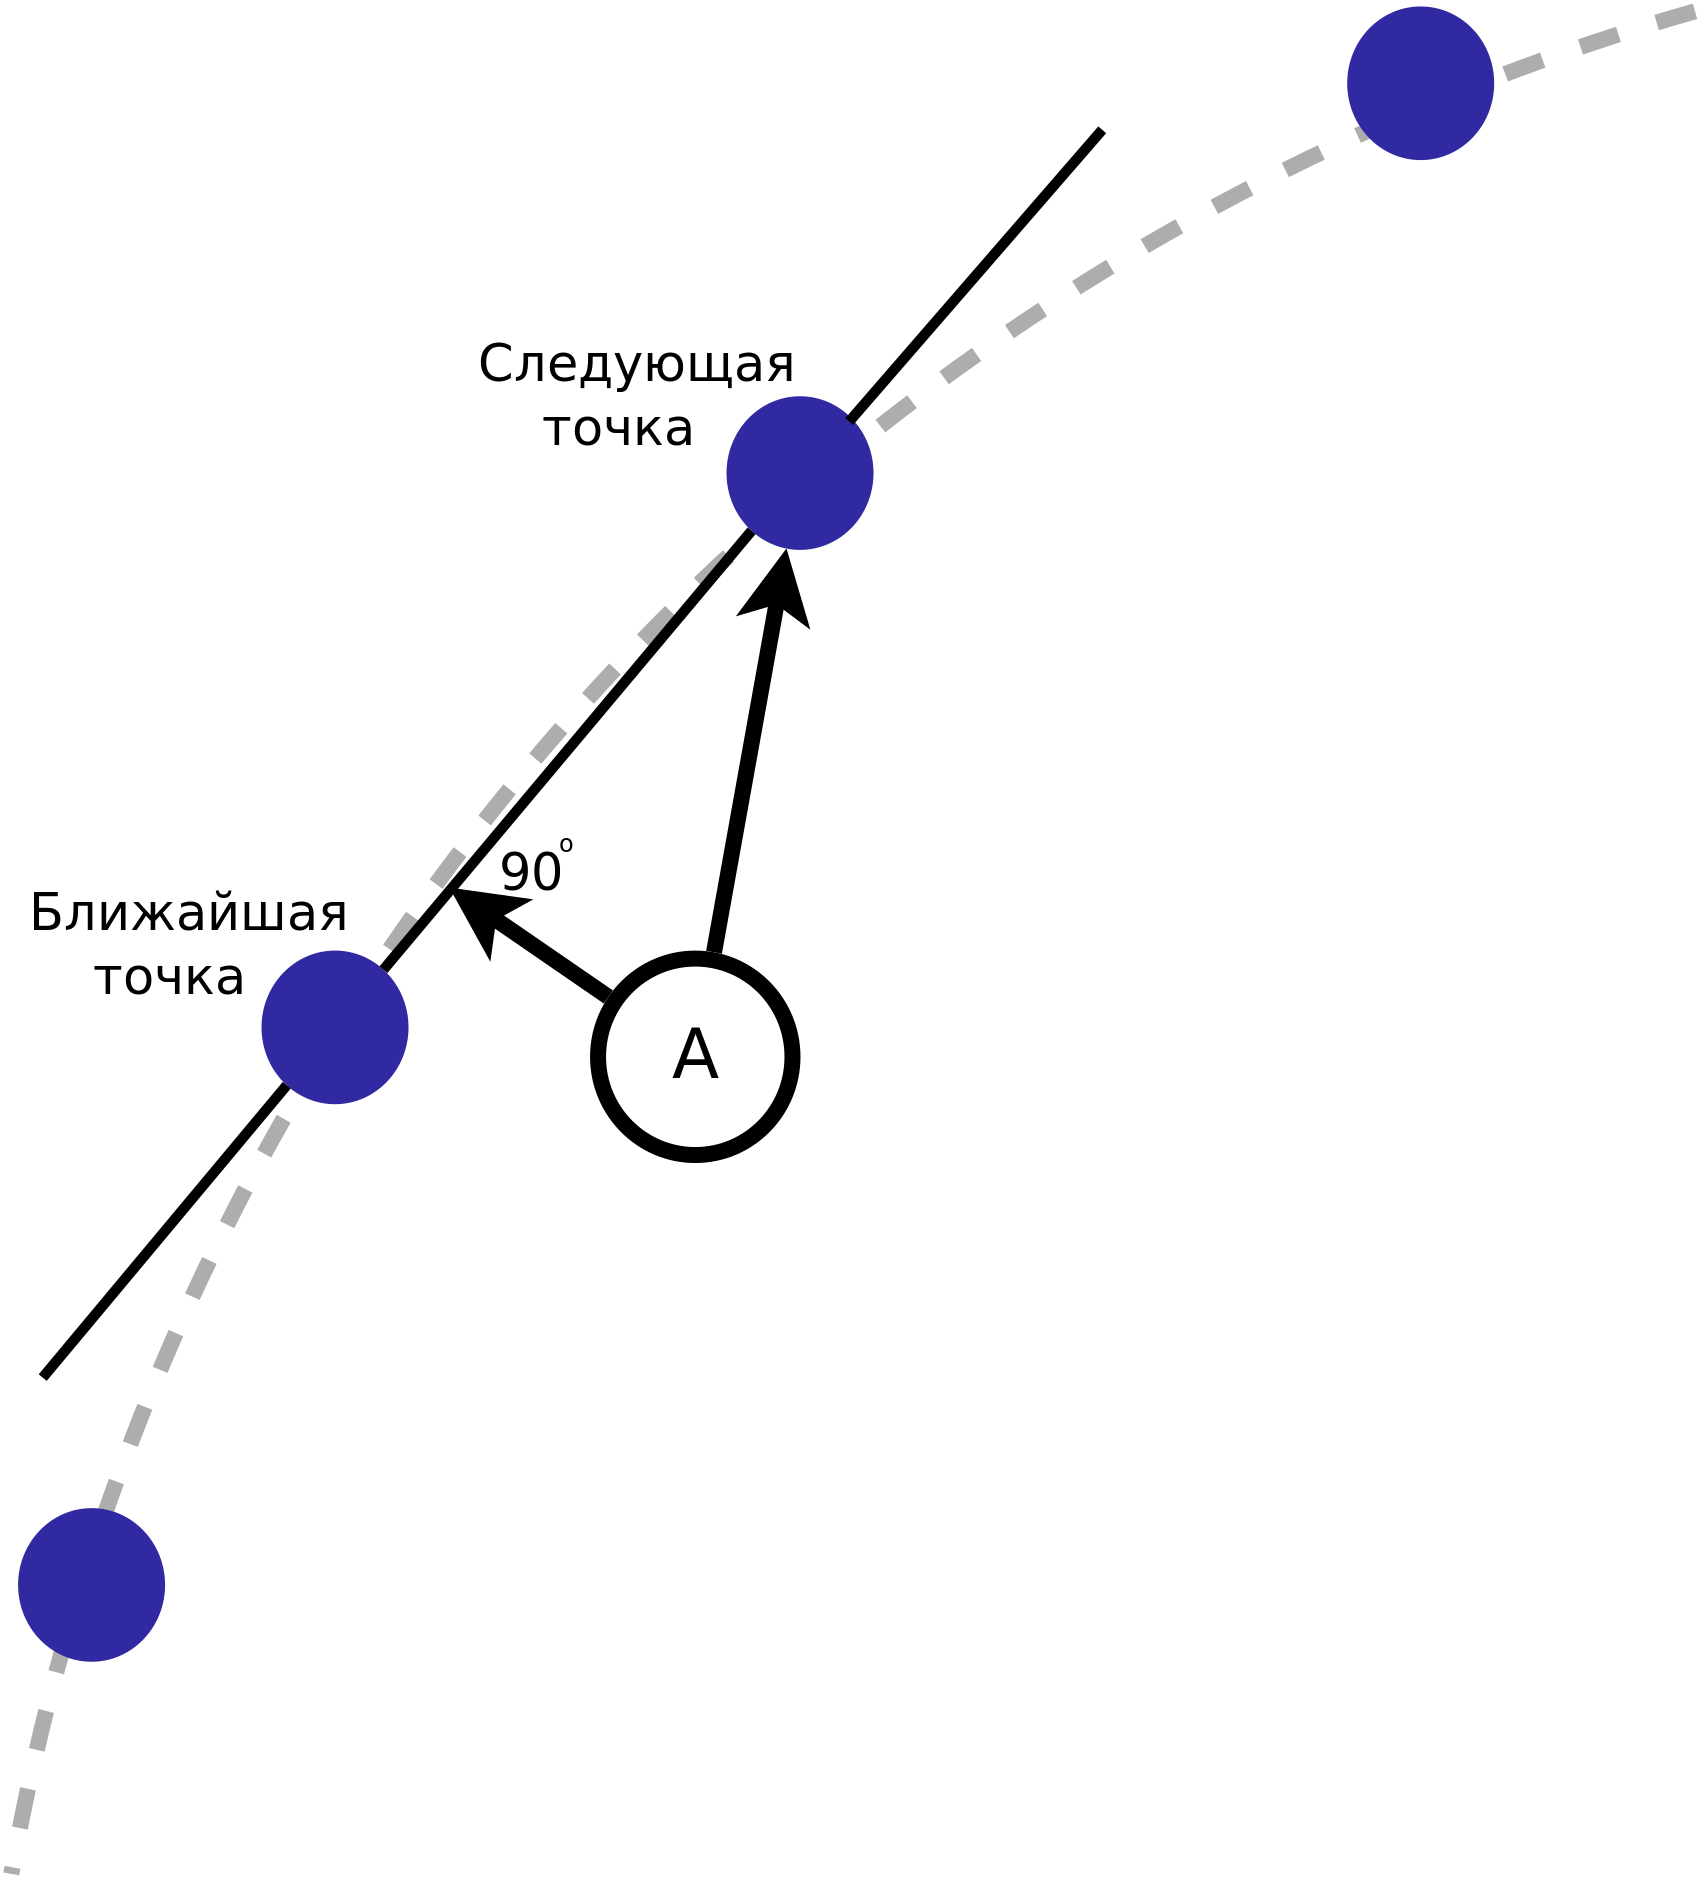
\includegraphics[width=0.6\linewidth]{others/master-alg}
	\caption{Поясняющий рисунок к алгоритму движения мастера по траектории}
	\label{fig:master-alg}
\end{figure}
\end{frame}

\begin{frame}[noframenumbering]
	Перемещения агентов при отказе второго агента находящегося во второй точке структуры.
	\begin{columns}
		\column{0.5\textwidth}
		\begin{figure}
			\centering
			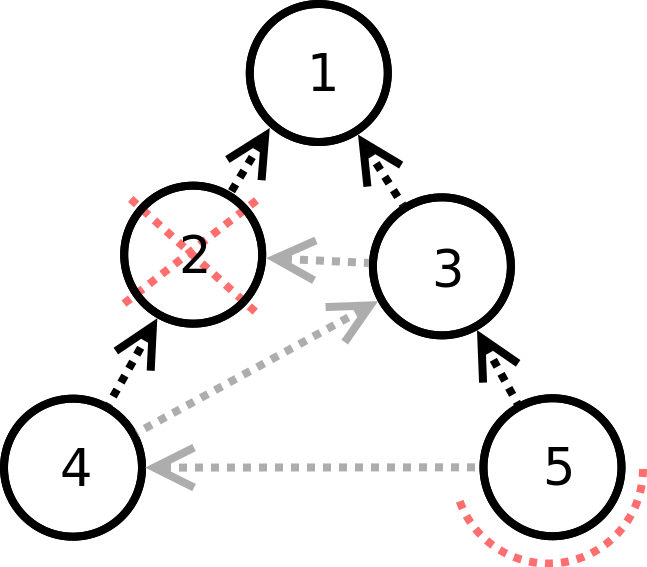
\includegraphics[width=1\linewidth]{platoon/agents-ordering-platoon}
			\caption{Точки структуры строя}
			\label{fig:agents-ordering-platoon}
		\end{figure}

		\column{0.5\textwidth}
		\begin{figure}
			\centering
			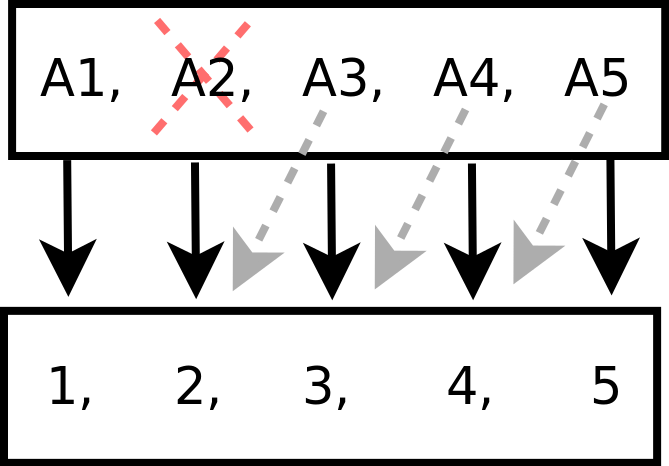
\includegraphics[width=1\linewidth]{platoon/agents-ordering}
			\caption{Отношения агент-точка структуры}
			\label{fig:agents-ordering}
		\end{figure}
		
	\end{columns}
\end{frame}
\begin{frame}[noframenumbering]
	
	\begin{figure}
		\centering
		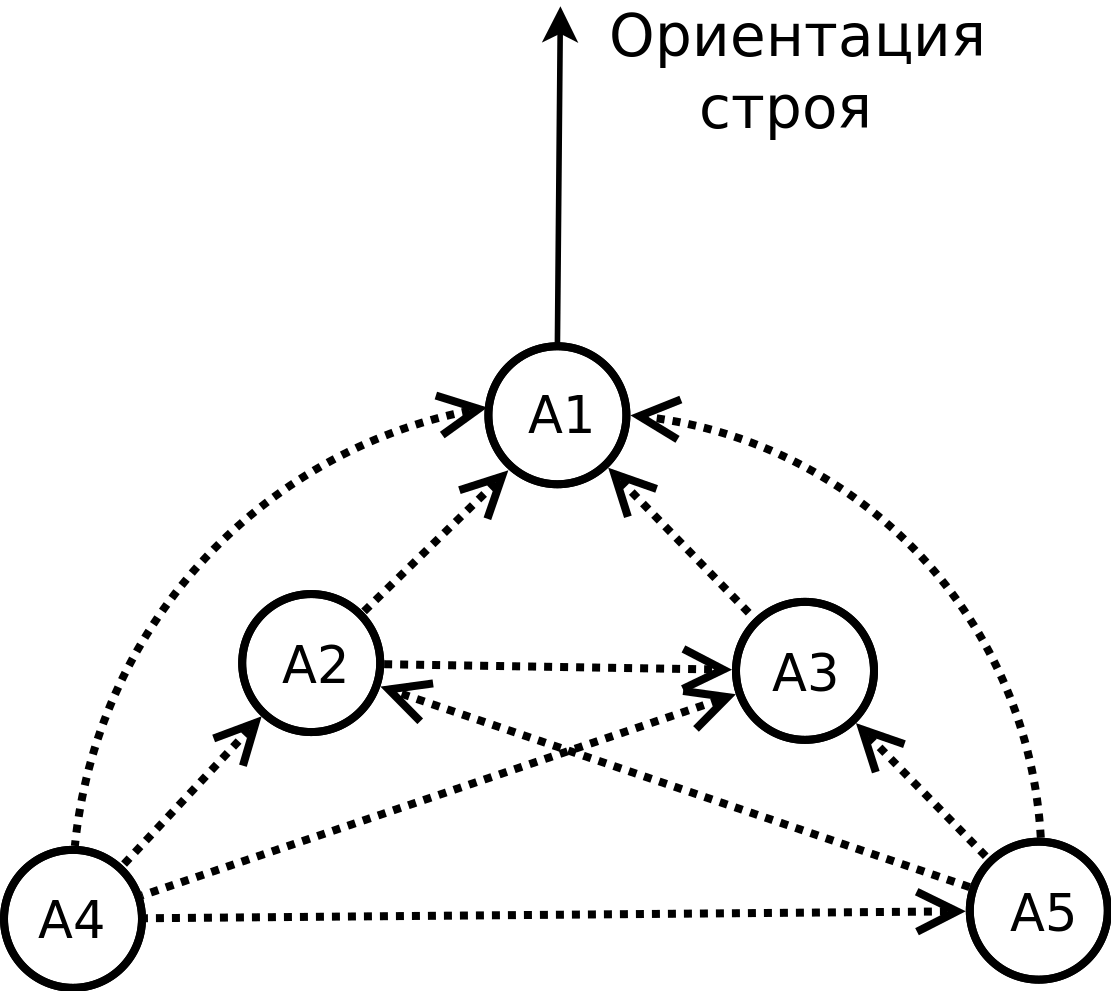
\includegraphics[width=0.7\linewidth]{platoon/wedge-platoon-full}
		\caption{Строй со всеми изображёнными связями}
		\label{fig:wedge-platoon-full}
	\end{figure}
\end{frame}
\begin{frame}[noframenumbering]
\begin{figure}
	\centering
	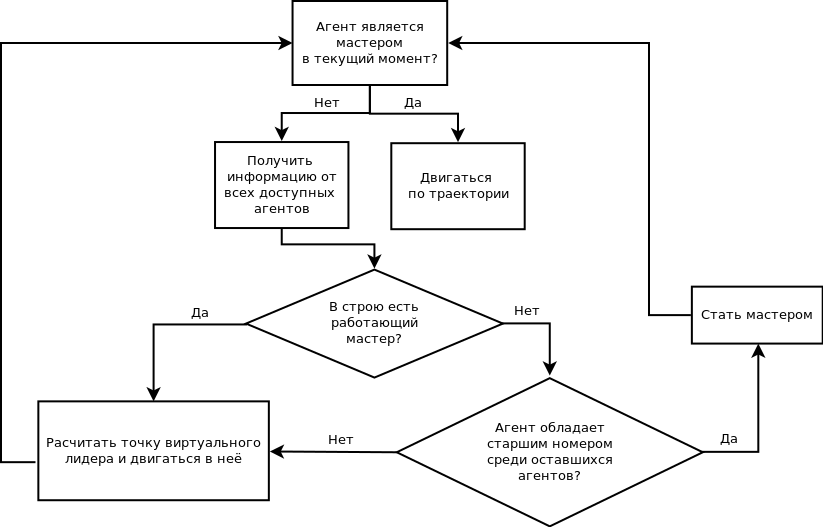
\includegraphics[width=1\linewidth]{others/algo-dia}
	\caption{Блок схема работы агента}
	\label{fig:algo-dia}
\end{figure}

\end{frame}

\end{document}
